\documentclass[10pt,a4paper]{article}
\usepackage[latin1]{inputenc}
\usepackage{amsmath}
\usepackage{amsfonts}
\usepackage{amssymb}
\usepackage{graphicx}
\usepackage[pdfauthor={Gergely Imreh},
            pdfsubject={Experimental atomic physics},
            pdftitle={The mode-locked laser CPT experiment}
            colorlinks=false
            ]{hyperref}
\setlength{\topmargin}{0in}
\setlength{\headheight}{0in}
\setlength{\headsep}{0in}
\setlength{\textheight}{7.7in}
\setlength{\textwidth}{6.5in}
\setlength{\oddsidemargin}{0in}
\setlength{\evensidemargin}{0in}
\setlength{\parindent}{0.25in}
\setlength{\parskip}{0.25in}
\title{The mode-locked laser CPT experiment}
\author{Gergely Imreh}
\date{\today}
\begin{document}
\maketitle

Earlier experimental results include \cite{Brandt1997}.
Detailed discussion of the buffer gas' effect on the CPT signal can be found in \cite{Erhard2001}.
Detailed analytical discussion of the CPT signal (all the levels) in \cite{Taichenachev2003}.
Invited paper about spectroscopy with CPT \cite{Taichenachev2003} (predates frequency comb but includes narrowing).

People investigate Rb in similar (but CW) situation. They find very low detuning induced shifts and very narrow linewidths. \cite{Erhard2000}.

Older theory and experiment, using extra RF field \cite{Vanier1998}.

Anoter... \cite{Vanier1998}

Buffer-gas induced absorption resonance, that is narrower than then the transmission resonance \cite{Mikhailov2004}. Buffer-gas enhances nonlinear effects??? We must have loads of that! More in \cite{Mikhailov2004,Lukin1997,Harris1999,Johnsson2002}. Most of the details there are about coherently enhanced 4-wave mixing (read more!), and some time the optical medium is the dense one, not the buffer gas (which is in practice transparent to our fields).

\section{Frequency combs}

\section{Buffer gas topics}

Apparently the buffer-gas issues are not completely resolved. As fart back as 1999 people still had contradictory results how the high pressure of different gasses affect the CPT signal. E.g. \cite{Gozzini1999} has some experiments on the subject, but mostly cited for the references within.

\section{Calculation techniques}

Collection of calculation tricks used in the literature.
Although for CW, this is interesting how do they calculate the expected CPT lineshape \cite{Novikova2005}

\section{Signal improvements}

\subsection{Overview}
  For the current simulation, the CPT signal is decribed as coherence slowly building up between ground-state levels. In absence of light, this coherence decays away. The decay rate is up for significant discussion, and might have influence on the outcome of the actual experiment.

  The time-dependent CPT signal is modelled as a decay of fluorescence as the ground-state coherence builds up. The upper-level transition and decay is assumed to be much faster.

\subsection{Calculation}
  This assumed waveform with properties of background levels (durin off-time andalso during on-time when off-resonance), system time constant (relative to chopping frequency) and lock-in phase (relative to the chopping frequency phase). The lock-in signal integral is taken from Wikipedia.

\subsection{Chopping near the characteristic frequency ($F_c \approx 1$)}
  High signal/background ratio can be achived by tuning the lock-in phase such that the background is nulled (in the simulation $\approx 86^{\circ}$ compared to the resonance). In other regions the $(S + B)/B \approx 1$, near that region it can be very high. The resonance is quite narrow, so might be difficult to hit.
  Also, under these circumstances the drop in the real signal actually increases the signal, this giving a peak! See Figure \ref{fig:chopphase1}.

\begin{figure}[h]
\centering
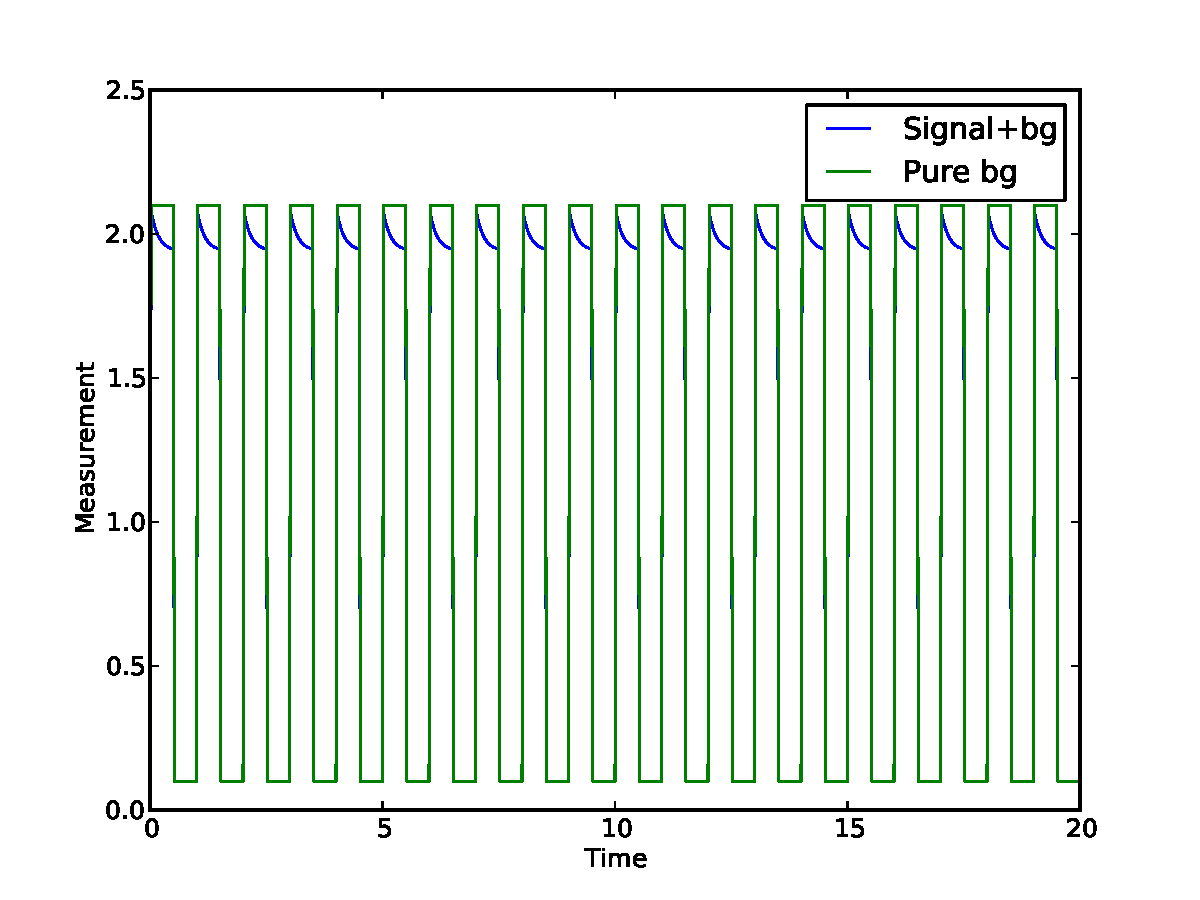
\includegraphics[width=0.6\textwidth]{figures/cpt01a.pdf}
\caption{Time-dependent signal at $F_c = 1$.}
\label{fig:choptime1}
\end{figure}
\begin{figure}[h]
\centering
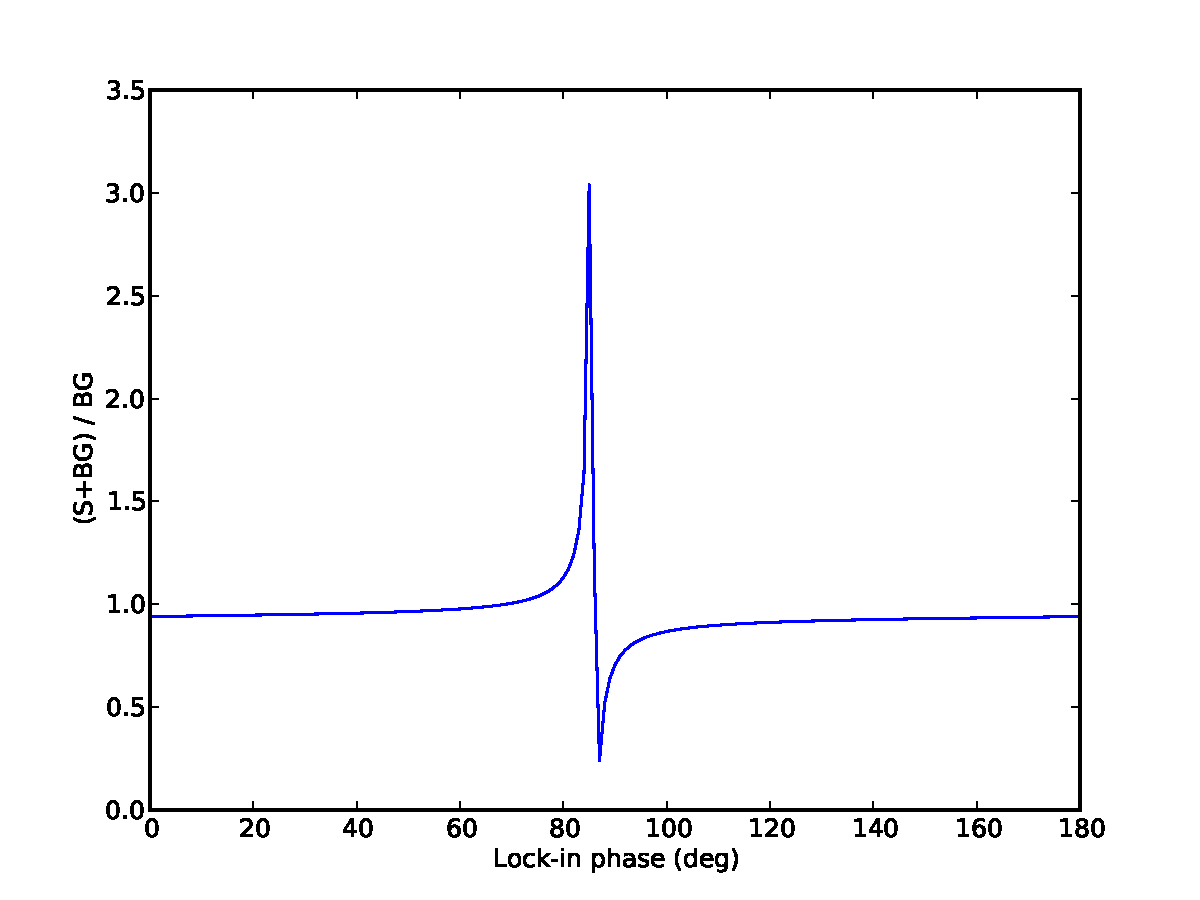
\includegraphics[width=0.6\textwidth]{figures/cpt01b.pdf}
\caption{Signal and background relationship for chopping at $F_c = 1$.}
\label{fig:chopphase1}
\end{figure}


\subsection{Low frequency chopping ($F_c \gg 1$)}
  Seems to only work on the other side of the resonance ($> \approx 86^{\circ}$), where a bigger drop is observed: $(S + B) / B \ll 1$.

\begin{figure}[h]
\centering
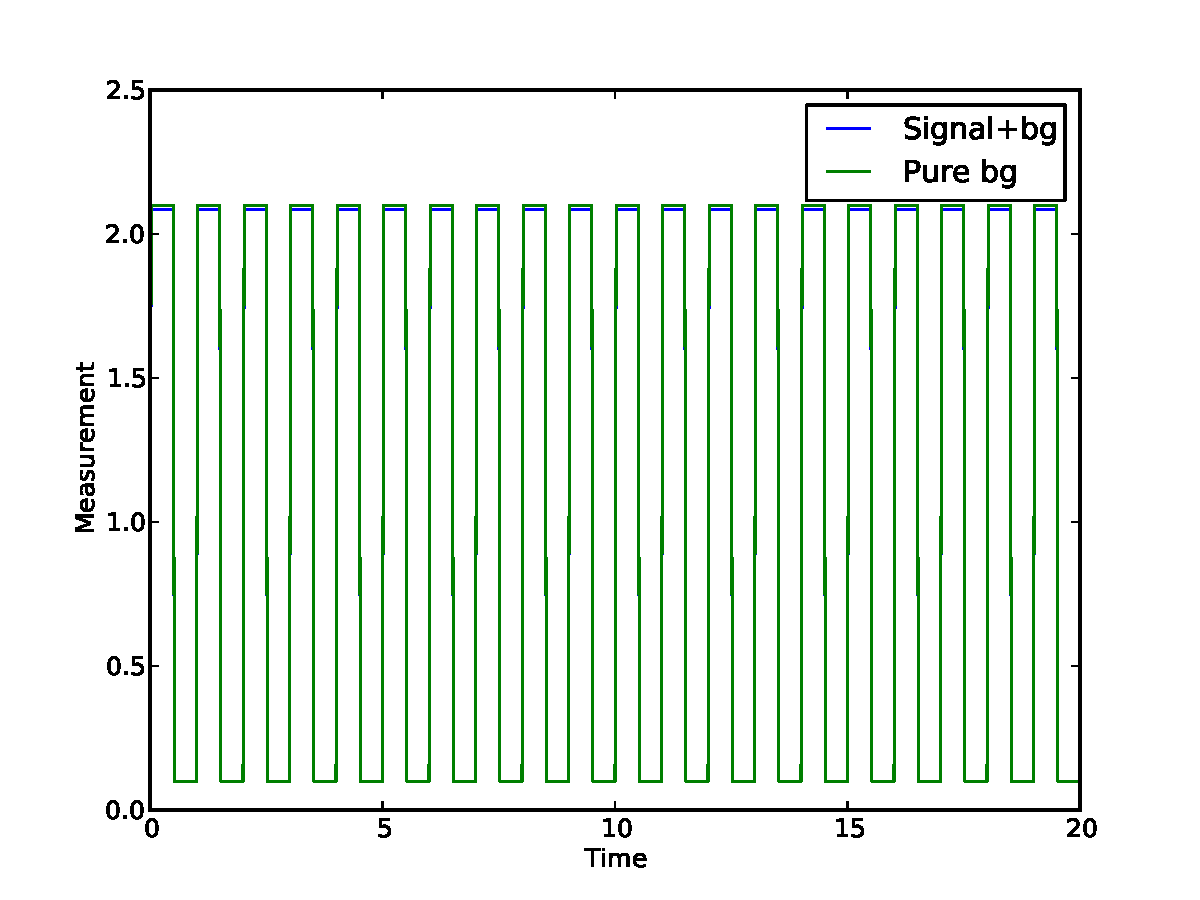
\includegraphics[width=0.6\textwidth]{figures/cpt02a.pdf}
\caption{Time-dependent signal at $F_c \gg 1$.}
\label{fig:choptime2}
\end{figure}
\begin{figure}[h]
\centering
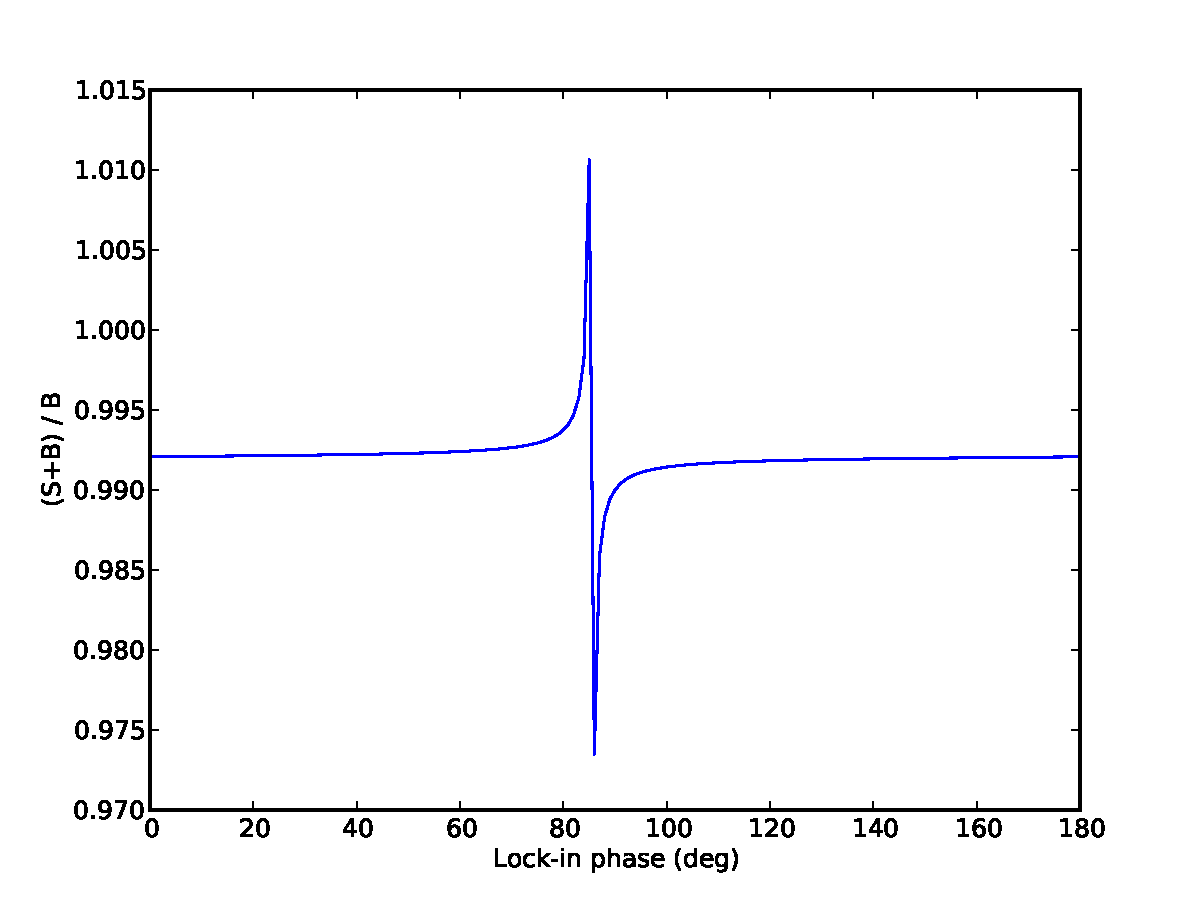
\includegraphics[width=0.6\textwidth]{figures/cpt02b.pdf}
\caption{Signal and background relationship for chopping at $F_c \gg 1$.}
\label{fig:chopphase2}
\end{figure}

\bibliographystyle{plain}
\bibliography{refs}
\end{document}
